\subsection{Group Functions}
SQL provides some simple aggregating functions that enable us to derive information about the rows in a table.

COUNT(*) \ \ \ \ returns a single value, the number of rows in the table

MAX(attribute) \ \ returns the largest value for the attribute

MIN(attribute) \ \ returns the smallest value for the attribute

AVG(attribute) \ \ works out the average value for this attribute

SUM(attribute)\ \ works out the total value for this attribute

They are called {\textquotedbl}group{\textquotedbl} functions because they take multiple rows of data, and output a single result.

\begin{center}
\begin{minipage}{2.501cm}
\begin{center}
\tablefirsthead{}
\tablehead{}
\tabletail{}
\tablelasttail{}
\begin{supertabular}{|m{2.3009999cm}|}
\hline
COUNT(*)\\\hline
5\\
\end{supertabular}
\end{center}
\end{minipage}
\end{center}
\ \ SELECT\ \ COUNT(*)

\ \  FROM\ \ CUST ;

{}- returns a single value, the number of rows in the customer table.

\ \ SELECT\ \ MIN(BALANCE)

\begin{center}
\begin{minipage}{3.692cm}
\begin{flushleft}
\tablefirsthead{}
\tablehead{}
\tabletail{}
\tablelasttail{}
\begin{supertabular}{|m{3.4919999cm}|}
\hline
MIN(BALANCE)\\\hline
.5\\
\end{supertabular}
\end{flushleft}
\end{minipage}
\end{center}
\ \ FROM\ \ \ \  ACC ;

Displays the lowest value held in the balance field from all the rows in the accounts table.

Any of these can be in an SQL statement that includes other clauses, e.g.:

\ \ SELECT\ \ COUNT(*)  AS {\textquotedbl}Sheffield Accounts{\textquotedbl}

\begin{center}
\begin{minipage}{3.942cm}
\begin{flushleft}
\tablefirsthead{}
\tablehead{}
\tabletail{}
\tablelasttail{}
\begin{supertabular}{|m{3.7419999cm}|}
\hline
Sheffield Accounts\\\hline
2\\
\end{supertabular}
\end{flushleft}
\end{minipage}
\end{center}
\ \ FROM \ \ CUST

\ \ WHERE \ \ AREA = {}`Sheffield' ;

{}- tells us how many customers are based in Sheffield.

For all of the following exercises you should check your results carefully against the table listings in the Introduction.

C1\ \ What are the lowest and highest basic salaries within the company?



\begin{center}
  
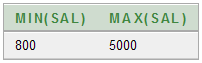
\includegraphics[width=5.415cm,height=1.658cm]{images/img (31).png}

\end{center}
\begin{flushleft}
\tablefirsthead{}
\tablehead{}
\tabletail{}
\tablelasttail{}
\begin{supertabular}{|m{10.082cm}|}
\hline
Select

\\\hline
\end{supertabular}
\end{flushleft}
C2\ \ How many people have a salary greater than £2000?

\begin{flushleft}
\tablefirsthead{}
\tablehead{}
\tabletail{}
\tablelasttail{}
\begin{supertabular}{|m{14.583cm}|}
\hline
Select count(*)

From

Where\\\hline
\end{supertabular}
\end{flushleft}
C3\ \ How many people are there in department 10?  

\begin{flushleft}
\tablefirsthead{}
\tablehead{}
\tabletail{}
\tablelasttail{}
\begin{supertabular}{|m{14.583cm}|}
\hline
Select

\\\hline
\end{supertabular}
\end{flushleft}
\subsection{NULL Values}
If a column has no value for any particular row, it is referred to as having a NULL value. This is not the same as a zero in a numeric column, nor a space in a character column.  NULL can be used in the same way as a numeric or character value.



\begin{center}
\begin{minipage}{4.849cm}
   

\includegraphics[width=4.341cm,height=4.341cm]{images/img (32).png}
 

   

\includegraphics[width=1.582cm,height=0.674cm]{images/img (15).png}
 
\end{minipage}
\end{center}
\ \ \ \ \ \ SELECT * from CUST where AREA IS NULL ;

\begin{flushleft}
\tablefirsthead{}
\tablehead{}
\tabletail{}
\tablelasttail{}
\begin{supertabular}{|m{1.9909999cm}|m{2.3009999cm}|m{2.0509999cm}|m{2.55cm}|m{1.8cm}|}
\hline
ACCNO &
BALANCE

 &
BRANCH &
OPENED &
BONUS\\
5418490 &
\raggedleft 1789.40 &
Broomhill &
6 May 1988 &
\centering\arraybslash {}-\\\hline
\end{supertabular}
\end{flushleft}
\ \ \ \ \ \ SELECT * from CUST where AREA IS NOT NULL ;

\begin{flushleft}
\tablefirsthead{}
\tablehead{}
\tabletail{}
\tablelasttail{}
\begin{supertabular}{|m{2.047cm}|m{2.3009999cm}|m{2.052cm}|m{2.425cm}|m{1.737cm}|}
\hline
ACCNO &
BALANCE &
BRANCH &
OPENED &
BONUS\\\hline
1245890 &
\raggedleft 234.50 &
Broomhill &
12 Nov 2003 &
\raggedleft\arraybslash 100.00\\
1494315 &
\raggedleft 0.50 &
Tinsley &
15 Dec 1999 &
\raggedleft\arraybslash 0.00\\
\end{supertabular}
\end{flushleft}
C4\ \ Run the following two statements

\ \ \ \ SELECT COUNT(*) from Emp ;

\ \ \ \ SELECT COUNT(Deptno) from Emp ;

\ \ Iidentify the difference in the results. What is the difference?  And why?

\begin{flushleft}
\tablefirsthead{}
\tablehead{}
\tabletail{}
\tablelasttail{}
\begin{supertabular}{|m{14.583cm}|}
\hline
\\\hline
\end{supertabular}
\end{flushleft}
count(*) counts all the selected rows, whereas a function that uses a specific column only uses the non-null values in that column, ignoring the null values.

C5\ \ List the employees with no commission recorded in their details.  

\begin{flushleft}
\tablefirsthead{}
\tablehead{}
\tabletail{}
\tablelasttail{}
\begin{supertabular}{|m{14.583cm}|}
\hline
Select

\\\hline
\end{supertabular}
\end{flushleft}
Hint:  if you check in the EMP table you should see that there are 10 such employees.  One employee has a zero commission, but that is a recorded value, and therefore should not be included in the count as it is not NULL.

\subsection{The NVL Function}
A further problem is that any calculation that includes a NULL value will always produce a NULL value.

\ \ \ \ \ \ NVL(column, replacement\_value)

The NVL function can be used to convert a null into a specified value i.e. it will return the actual value of the specified column if it has a value, or the replacement value if the column is null.  This is often necessary when performing calculations, or formatting for output since null values will be totally ignored by many functions and operations.  This may be applied to a column of any data type provided the replacement value is of the same type as the column.

\ \ SELECT \ \ ACCNO,

\ \ \ \ \ \ NVL(BONUS, 0)

\begin{center}
\begin{minipage}{6.442cm}
\begin{flushleft}
\tablefirsthead{}
\tablehead{}
\tabletail{}
\tablelasttail{}
\begin{supertabular}{|m{2.4919999cm}|m{3.5479999cm}|}
\hline
ACCNO &
NVL(BONUS, 0)\\\hline
5418490 &
0\\
\end{supertabular}
\end{flushleft}
\end{minipage}
\end{center}
\ \ from ACC

\ \ where BONUS IS NULL ;

C6\ \ List the name, job and commission for all employees, replacing the commission with a 0 for employees that have none.

\begin{center}
\begin{minipage}{4.849cm}
   

\includegraphics[width=4.341cm,height=4.341cm]{images/img (33).png}
 

   

\includegraphics[width=1.582cm,height=0.674cm]{images/img (15).png}
 
\end{minipage}
\end{center}
\begin{flushleft}
\tablefirsthead{}
\tablehead{}
\tabletail{}
\tablelasttail{}
\begin{supertabular}{|m{11.142cm}|}
\hline
Select

\\\hline
\end{supertabular}
\end{flushleft}
C7\ \ Change C6 to list the name, job and total income (salary + commission) for all employees.  Ensure the total income is shown for all employees, including those without commission.

\begin{flushleft}
\tablefirsthead{}
\tablehead{}
\tabletail{}
\tablelasttail{}
\begin{supertabular}{|m{11.08cm}|}
\hline
Select

\\\hline
\end{supertabular}
\end{flushleft}
C8\ \ What are the highest and lowest incomes (including commission) for all employees?

\begin{flushleft}
\tablefirsthead{}
\tablehead{}
\tabletail{}
\tablelasttail{}
\begin{supertabular}{|m{14.583cm}|}
\hline
Select

\\\hline
\end{supertabular}
\end{flushleft}
C9\ \ What is the total income (one value) of those employees who have been allocated commission (a commission value is recorded)?

\begin{flushleft}
\tablefirsthead{}
\tablehead{}
\tabletail{}
\tablelasttail{}
\begin{supertabular}{|m{14.583cm}|}
\hline
Select

\\\hline
\end{supertabular}
\end{flushleft}
\subsection{The GROUP BY clause}
The GROUP BY clause splits the table into specified groups according to the criteria specified, returning one summary row for each group.

The following will list the sum of the account balances for each branch.

 SELECT \ \ BRANCH,

\begin{center}
\begin{minipage}{4.692cm}
\begin{flushleft}
\tablefirsthead{}
\tablehead{}
\tabletail{}
\tablelasttail{}
\begin{supertabular}{|m{2.4919999cm}|m{1.798cm}|}
\hline
BRANCH &
TOTAL\\\hline
Broomhill &
2023.9\\\hline
Tinsley &
.5\\
\end{supertabular}
\end{flushleft}
\end{minipage}
\end{center}
\ \ \ \ SUM(BALANCE) AS TOTAL

FROM\ \  \ \ ACC 

GROUP BY \ \ BRANCH ;

Only specify columns in the SELECT clause if they are in the grouping clauses or are functions (SUM, MIN, etc); otherwise syntax errors will occur.  Similarly, it would be rather pointless to display a total without saying what it refers to (i.e. Branch), therefore specify ALL grouping columns in the SELECT clause.

C10\ \ What would be the result of the following query?  You can't run the code; you should work out the expected result using the printout of the data p. 7.



\begin{center}
\begin{minipage}{4.849cm}
   

\includegraphics[width=4.341cm,height=4.341cm]{images/img (34).png}
 

   

\includegraphics[width=1.582cm,height=0.674cm]{images/img (15).png}
 
\end{minipage}
\end{center}
SELECT \ \ AREA, COUNT(*)

FROM \ \ CUST

GROUP BY\ \ AREA ;

\begin{flushleft}
\tablefirsthead{}
\tablehead{}
\tabletail{}
\tablelasttail{}
\begin{supertabular}{|m{10.445001cm}|}
\hline
Expected result:

\\\hline
\end{supertabular}
\end{flushleft}
We can also specify levels of grouping, by stating more than one column to group by

\ \ SELECT \ \ BRANCH,

\begin{center}
\begin{minipage}{7.003cm}
\begin{flushleft}
\tablefirsthead{}
\tablehead{}
\tabletail{}
\tablelasttail{}
\begin{supertabular}{|m{2.2389998cm}|m{2.55cm}|m{1.6129999cm}|}
\hline
BRANCH &
OPENED &
TOTAL\\\hline
Broomhill &
12-NOV-03 &
2023.9\\\hline
Tinsley &
15-DEC-99 &
.5\\\hline
Broomhill &
06-MAY-88 &
1789.4\\
\end{supertabular}
\end{flushleft}
\end{minipage}
\end{center}
\ \ \ \ \ \ OPENED,

\ \ \ \ \ \ SUM(BALANCE) AS TOTAL

\ \ FROM\ \  \ \ ACC 

\ \ GROUP BY \ \ BRANCH,

\ \ \ \ \ \ OPENED ;

C11\ \ How many people are there in each department?

\begin{flushleft}
\tablefirsthead{}
\tablehead{}
\tabletail{}
\tablelasttail{}
\begin{supertabular}{|m{14.583cm}|}
\hline
Select

From

Group By

\\\hline
\end{supertabular}
\end{flushleft}
C12 \ \ How many people are there in each type of job within each department?

\begin{flushleft}
\tablefirsthead{}
\tablehead{}
\tabletail{}
\tablelasttail{}
\begin{supertabular}{|m{14.583cm}|}
\hline
Select

\\\hline
\end{supertabular}
\end{flushleft}
C13\ \ For each department, find the average salary and the total salary bill excluding commission. 

\begin{flushleft}
\tablefirsthead{}
\tablehead{}
\tabletail{}
\tablelasttail{}
\begin{supertabular}{|m{14.583cm}|}
\hline
Select

\\\hline
\end{supertabular}
\end{flushleft}
C14\ \ For each department, find the maximum commission earned, and the number of people in that department.

\begin{flushleft}
\tablefirsthead{}
\tablehead{}
\tabletail{}
\tablelasttail{}
\begin{supertabular}{|m{14.583cm}|}
\hline
Select

\\\hline
\end{supertabular}
\end{flushleft}
The HAVING clause

The HAVING clause is used to specify which GROUPS are to be used by the SELECT clause to generate the output by applying criteria to the results of grouping.

The WHERE clause restricts which rows are input to the full SELECT statement whereas the HAVING clause restricts which groups are to be used for output.  

Example: \ \ SELECT \ \ AREA, COUNT(REFNO) Customers

FROM \ \ CUST

\begin{center}
\begin{minipage}{4.849cm}
   

\includegraphics[width=4.341cm,height=4.341cm]{images/img (35).png}
 

   

\includegraphics[width=1.582cm,height=0.674cm]{images/img (15).png}
 
\end{minipage}
\end{center}
GROUP BY\ \ AREA

HAVING\ \ COUNT(REFNO) {\textgreater} 1 ;

C15\ \ Check the data p.7, and write down what the results of the previous query would be.

\begin{flushleft}
\tablefirsthead{}
\tablehead{}
\tabletail{}
\tablelasttail{}
\begin{supertabular}{|l|l|}
\hline
 & \\\hline
 & \\\hline
\end{supertabular}
\end{flushleft}
C16\ \ Display the department number and number of employees in departments with 5 or more employees. 

\begin{flushleft}
\tablefirsthead{}
\tablehead{}
\tabletail{}
\tablelasttail{}
\begin{supertabular}{|m{14.583cm}|}
\hline
Select

From

Group By

Having\\\hline
\end{supertabular}
\end{flushleft}
Note: The GROUP BY clause sets the sort order of the selected rows.  The rows are in ascending order, for each of the GROUP BY columns, in order.  Where this is not what is required, control the sequence of selected rows by

\begin{center}
  

\includegraphics[width=1.06cm,height=0.903cm]{images/img (2).png}

\end{center}
 using an ORDER BY clause in addition to a GROUP BY clause.

C17\ \ Display in descending value, the average salary for those jobs held by two or more people.

\begin{flushleft}
\tablefirsthead{}
\tablehead{}
\tabletail{}
\tablelasttail{}
\begin{supertabular}{|m{14.583cm}|}
\hline
Select

\\\hline
\end{supertabular}
\end{flushleft}
In the logic of SQL, \ \ WHERE \ \ is processed before

\ \ \ \ \ \ GROUP BY \ \ is processed before

\ \ \ \ \ \ HAVING.
